\documentclass{report}

\usepackage{tikz}
\usetikzlibrary{calc,trees,positioning,arrows,chains,shapes.geometric,%
    decorations.pathreplacing,decorations.pathmorphing,shapes,%
    matrix,shapes.symbols}
\tikzset{
>=stealth',
  graphnode/.style={
    rectangle, 
    rounded corners, 
    % fill=black!10,
    draw=black, very thick,
    text width=10em, 
    minimum height=3em, 
    text centered, 
    on chain},
  line/.style={draw, thick, <-},
  element/.style={
    tape,
    top color=white,
    bottom color=blue!50!black!60!,
    minimum width=8em,
    draw=blue!40!black!90, very thick,
    text width=10em, 
    minimum height=3.5em, 
    text centered, 
    on chain},
  every join/.style={->, thick,shorten >=1pt},
  decoration={brace},
  hsplit/.style={decorate}
}

\begin{document}

\title{CoreConstraint Documentation \\ \large The theory behind the CoreConstraint solver}
\author{Blake Loring}
\date{\today}

\maketitle

\chapter {Introduction}

CoreConstraint is designed to be a simplistic, integer only, abstract constraint solver. Allowing CoreVM to have a simple interface to a constraint solver which can verify whether a path is satisfiable by looking at path constraints.

\chapter {Constraint Solvers}

A constraint solver is a piece of software that can take a set of constraints (Such as X > 50, Y < 40, X + Y = 60, X > 0, Y > 0) and find out A. if there is some allocation of variables which satisfies them and B. An allocation of variables which satisfies them.

\chapter {Theory}

The CoreConstraint constraint solver only has to be able to be able to verify linear, integer only constraints. In order to do this the constraints problem is modeled as a optimization problem and then solved using the Simplex algorithm.

\chapter {Implementation}

The constraints solver comes in two parts, the simplified interface used to construct a problem definition (Constraints::Problem) and the solver (Simplex::Table, Simplex::Solver).

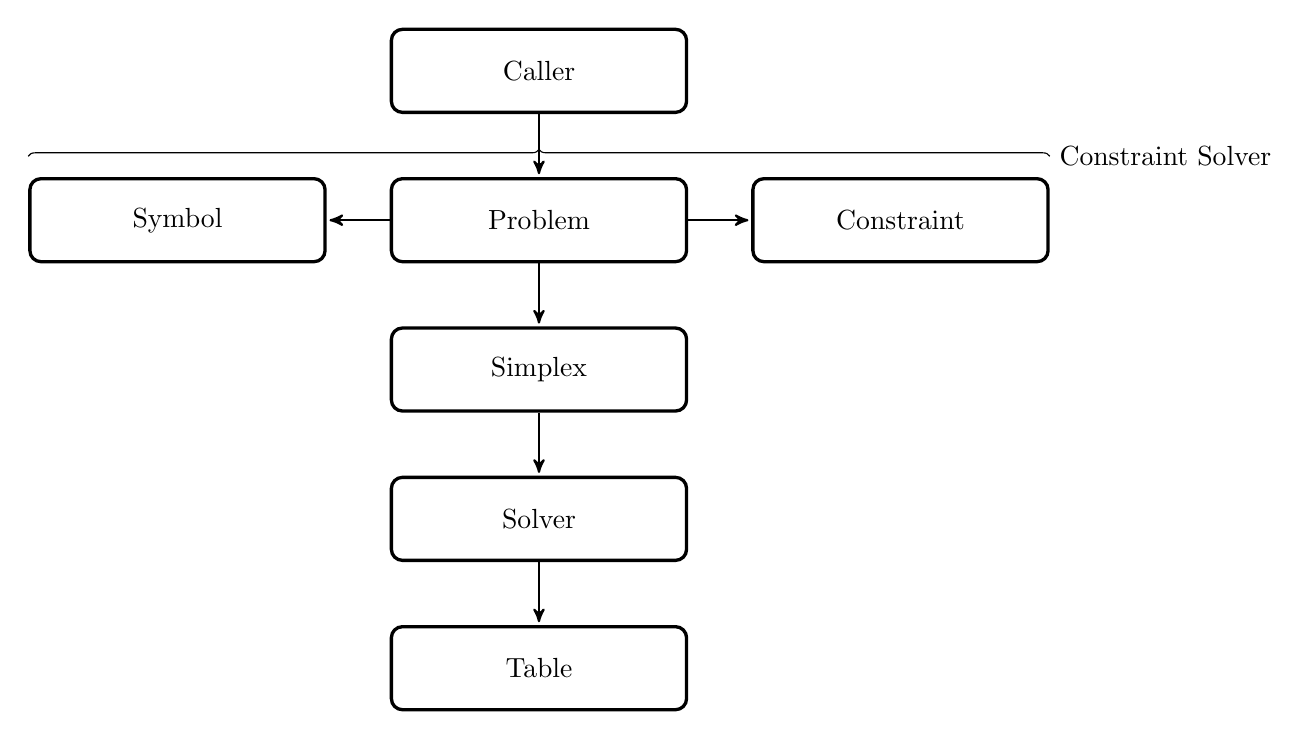
\begin{tikzpicture}
  [node distance=.8cm,
  start chain=going below,]
  \node[graphnode, join] {Caller};
  \node[graphnode, join] (Problem) {Problem};
  \begin{scope}[start branch=venstre]
    \node[graphnode, on chain=going left, join] (Symbol) {Symbol};
  \end{scope}
  \begin{scope}[start branch=venstre]        
    \node[graphnode, on chain=going right, join] (Constraint) {Constraint};
  \end{scope}

  \node[graphnode, join] (Simplex) {Simplex};
  \node[graphnode, join] (Solver) {Solver};
  \node[graphnode, join] (Table) {Table};

  \draw[hsplit] let
    \p1=(Symbol.west), \p2=(Constraint.east), \p3=(Problem.north) in ($(\x1,\y3+.75em)$) -- ($(\x2,\y3+.75em)$) node[above, right]  {Constraint Solver};
\end{tikzpicture}

\chapter {Results}
\chapter {Conclusion}

\end{document}
